\section{Transformer}
\label{sec:transformer}

Transformer sind erweiterte Deep-Learning-Modelle, welche sich aus einem Encoder und einem Decoder zusammensetzen (siehe Abbildung 
\ref{fig:transformeroverview}) und den sogenannten Self-Attention Mechanismus nutzen \cite{vaswani2023attentionneed}.

\begin{figure}[htbp]
    \begin{center}
        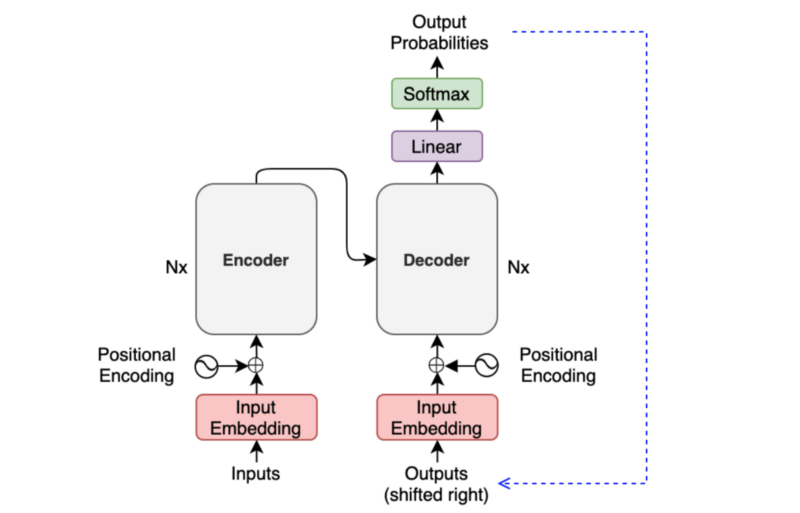
\includegraphics[scale=0.4]{static/transformer-overview.png}
        \caption{\label{fig:transformeroverview} Eine Übersicht der Transformer Architektur \cite{kikaben2021transformer} 
        - vereinfacht von \cite{vaswani2023attentionneed}}
    \end{center}
\end{figure}

Im Vergleich zu RNNs, welche Kontexte nur von links nach rechts erkennen können (bzw. bi-direktional in BiLSTMs) kann der Kontext in Transformern
global erkannt werden \cite{ghojogh2020}.

\subsection{Grundlagen der Transformer Architektur}

\subsubsection{Self-Attention} \label{sec:self_attention}

In \cite{vaswani2023attentionneed} wird die für Transformer entwickelte Self-Attention vorgestellt.
Diese ermöglicht es, Beziehungen zwischen verschiedenen Positionen innerhalb einer einzigen Sequenz zu modellieren. 
Jede Position, also z.B. ein Wort in einem Satz, kann dabei auf alle anderen Positionen achten, um eine neue Darstellung der Sequenz zu erzeugen, 
die globale Abhängigkeiten widerspiegelt.

In dem Satz „Die Bank hat heute geschlossen.“ erkennt Self-Attention zum Beispiel, dass „Bank“ im Kontext von „geschlossen“ eher ein Gebäude 
und kein Möbelstück ist.

Folgende Schritte erklären, wie Self-Attention laut \cite{vaswani2023attentionneed} funktioniert:

\begin{enumerate}
    \item \textbf{Einbettungen als Vektoren:} \\
    Jede Position der Eingabesequenz wird in einen Vektor eingebettet.

    \item \textbf{Erzeugung von Query, Key, Value (Q, K, V):} \\
    Aus diesen Vektoren werden durch lineare Transformationen die Matrizen \textit{Q (Query)}, \textit{K (Key)} und \textit{V (Value)} erzeugt.

    \item \textbf{Berechnung der Aufmerksamkeitsgewichte:} \\
    Die Self-Attention berechnet für jede Position die Kompatibilität zu allen anderen, indem die Skalarprodukte von $Q$ und $K$ gebildet und durch $\sqrt{d_k}$ skaliert werden:
    \[
    \text{Attention}(Q, K, V) = \text{softmax}\left(\frac{QK^T}{\sqrt{d_k}}\right) V
    \]
    Diese Softmax-Gewichte bestimmen, wie stark eine Position auf andere achten soll.

    \item \textbf{Neues Repräsentationsvektor:} \\
    Die gewichteten Werte ($V$) werden aufsummiert und bilden so eine neue Darstellung für jede Position. 
\end{enumerate}

Statt nur eine Self-Attention zu berechnen, verwenden Transformer mehrere parallele \textit{Heads}. Jeder \textit{Head} lernt eine andere Perspektive auf die Sequenz. 
Die Ergebnisse aller \textit{Heads} werden anschließend in einem \textit{MultiHead} kombiniert:

\begin{equation}
   \text{MultiHead}(Q, K, V) = \text{Concat}(\text{head}_1, \ldots, \text{head}_h) W^O 
\end{equation}


\subsubsection{Encoder-Decoder-Architektur} \label{sec:encoder_decoder_architecture}

Ein Encoder-Decoder-Modell wird verwendet, um eine Eingabesequenz in eine Ausgabesequenz umzuwandeln. 
Zum Beispiel würde bei einer Textübersetzung der Encoder die Eingabesequenz sprachlich verstehen und der Decoder den übersetzten Text der Ausgabesequenz generieren.

Der Encoder nimmt eine Folge von Eingabewörtern und wandelt sie in eine Reihe von Vektoren um, die Informationen über jedes Wort und dessen Zusammenhang enthalten.

In der ursprünglichen Version der Encoder-Decoder-Architektur werden hierfür Recurrent Neural Networks (RNNs) oder bidirektionale RNNs verwendet.
Diese lesen die Eingabe von vorne und hinten \cite{bahdanau2016neuralmachinetranslationjointly}.

Im von \cite{vaswani2023attentionneed} vorgestelltem Transformer-Modell werden RNNs durch Self-Attention ersetzt. 


\subsubsection{Hidden Layer} \label{sec:hidden_layer}

In einem Transformer-Modell \cite{vaswani2023attentionneed} bestehen die \textit{hidden layers} aus mehreren Encoder- und/oder Decoder-Schichten.
Die erste Schicht erhält den Input und die letzte Schicht gibt den Output aus. Alle anderern Schichten sind versteckt und werden
als \textit{hidden layer} bezeichnet.

Im Falle eines Encoding Transformers wie BERT (siehe Kapitel \ref{sec04:bert}) funktionieren \textit{hidden layer} wie folgt \cite{DBLP:journals/corr/abs-1810-04805}:

\begin{enumerate}
    \item \textbf{Input-Einbettung:} Jeder Token wird in einen Zahlenvektor umgewandelt. 
    Zusätzlich werden Positions- und Segmentinformationen hinzugefügt.
    
    \item \textbf{Verarbeitung durch Hidden Layers:} 
    \begin{itemize}
        \item Jedes \textit{hidden Layer} ist ein Transformer-Block mit Self-Attention.
        \item Jeder Token wird an allen anderen Tokens angepasst, um seine Bedeutung im Kontext zu erfassen.
        \item Diese Aufmerksamkeit ist bidirektional – sie bezieht sich auf Wörter davor und danach.
    \end{itemize}
    
    \item \textbf{Tiefe Verfeinerung:} 
    \begin{itemize}
        \item Frühe Schichten lernen einfache Beziehungen (z.B. Wortpaare, Syntax).
        \item Spätere Schichten modellieren komplexere Abhängigkeiten (z.B. Bedeutung, logische Zusammenhänge).
    \end{itemize}
    
    \item \textbf{Ergebnis:} 
    \begin{itemize}
        \item Das letzte \textit{hidden Layer} liefert eine kontext-sensitive Repräsentation für jeden Token.
        \item In diesem Fall kann diese für Aufgaben wie Klassifikation, Fragebeantwortung oder Named Entity Recognition verwendet werden.
    \end{itemize}
\end{enumerate} 


\subsection{Transformer Modelle}
\label{sec:transformer_modelle}

\subsubsection{BERT} \label{sec04:bert}

Bidirectional Encoder Representations from Transformers (BERT) ist ein reiner, für Sprachverständnis optimierter, Encoder-Transformer \cite{devlin2019}.
Zwei wichtige Bestandteile der BERT Architektur sind die \textit{Self Attention Heads} und die \textit{Hidden Layers}
(siehe Kapitel \ref{sec:self_attention} und Kapitel \ref{sec:hidden_layer}).

Während CNNs und RNNs externe Word Embeddings wie Word2Vec oder GloVe verwenden, nutzt BERT eigene lernbare Embeddings.

Dazu noch einmal das Beispiel aus Kapitel \ref{sec:word_embeddings}: „Ich setze mich auf die Bank.“ und „Ich raube die Bank aus.“:

GloVe und Word2Vec erstellen einen festen Vektor für das Wort „Bank“, egal in welchem Satz es steht.
Bei GloVe ist dieser Vektor ein Mittelwert aus allen Bedeutungen, die „Bank“ im Korpus je hatte.
Der Vektor liegt folglich irgendwo zwischen Sitzmöbel und Finanzinstitut und repräsentiert keine der beiden Bedeutungen exakt.

BERT löst dieses Problem indem es kontextabhängige Embeddings erzeugt. So wird ein Vektor für das Wort „Bank“ erzeugt, der zur Bedeutung
Sitzmöbel passt und ein weiterer für die Bedeutung Finanzinstitut.

Es verwendet während des Trainings Masked Language Modeling (MLM), um den Kontext und die Bedeutung von Wörtern im Satz zu verstehen.
Anschließend wird es auf einem Datensatz mit gelabelten Bewertungen feinjustiert. 
Dabei verbindet es jedes Eingabeelement mit jedem Ausgabeelement und 
weist dabei wichtigen Wörtern und Phrasen im Text höhere Gewichtungen zu \cite{Deshai:2023aa}.

Im MLM wird ein bestimmer Teil der Wörter in der Eingabesequenz zufällig maskiert (siehe Abbildung \ref{fig:mlm_bert}), 
und das Modell muss diese verdeckten Wörter korrekt vorhersagen.

\begin{figure}[htbp]
    \begin{center}
        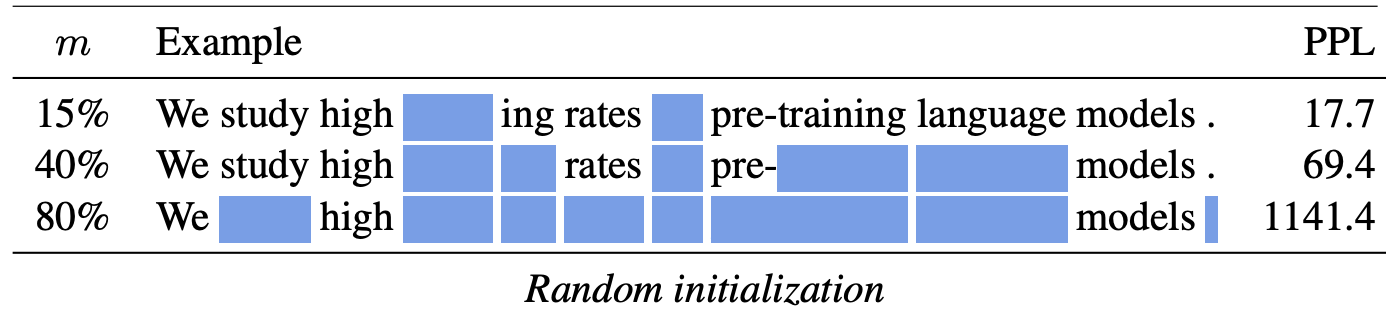
\includegraphics[scale=0.5]{static/mlm_bert.png}
        \caption{\label{fig:mlm_bert} Bsp. zum MLM \cite{wettig2023}}
    \end{center}
\end{figure}

BERT nutzt die bi-direktionale Transformer-Architektur (siehe Abbildung \ref{fig:architecture_bert}), bei welcher tiefe semantische Informationen 
eines Satzes erfasst werden können. Aufgrund dieser Bidirektionalität ist das Modell bei späteren Vorhersagen effektiver \cite{wettig2023}. 
\cite{devlin2019} zeigt, wie relevant bidirektionalen Pretrainings für qualitativ hochwertige Sprachrepräsentationen sind.

\begin{figure}[htbp]
    \begin{center}
        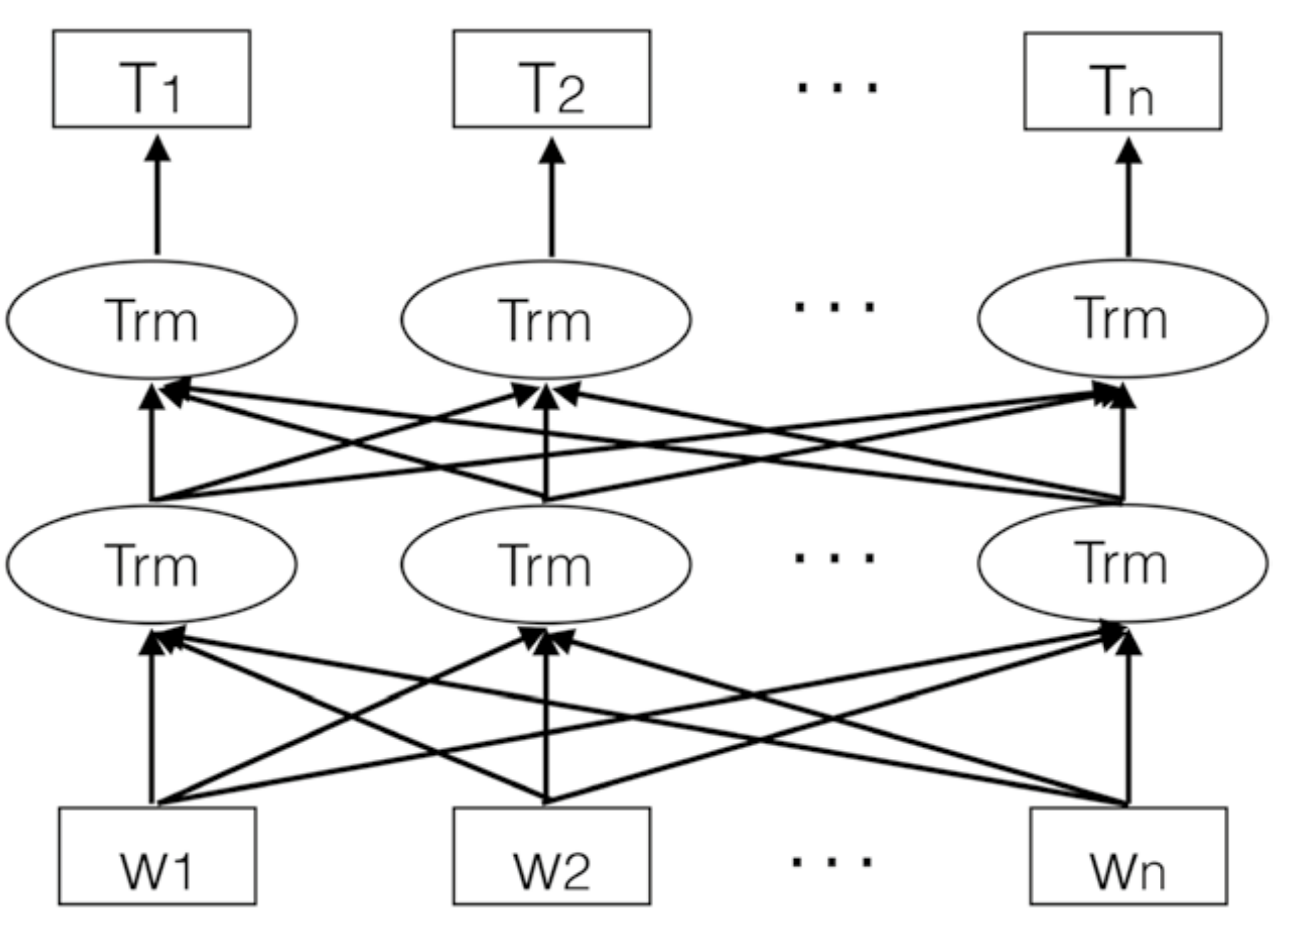
\includegraphics[scale=0.3]{static/architecture_bert.png}
        \caption{\label{fig:architecture_bert} Bidirektionalität des BERT Modells \cite{Wang:2020aa}}
    \end{center}
\end{figure}

Für das Erstellen der Wortvektoren nutzt BERT WordPiece Embeddings.
WordPiece ist ein Tokenisierungsverfahren, das Wörter in kleinere Einheiten zerlegt.
Es wurde von Google speziell für BERT entwickelt, um auch seltene oder unbekannte Wörter sinnvoll verarbeiten zu können.

Folgendes Beispiel für ein WordPiece Embedding (aus \cite{huggingface2025wordpiece}):
\begin{enumerate}
    \item Das \textbf{Startvokabular} besteht aus einem Vokabular aus Einzelbuchstaben 
    (z.B. \texttt{h}, \texttt{\#\#e}, \texttt{\#\#l}, \texttt{\#\#o} für ``hello''), 
    wobei alle Buchstaben außer dem Ersten mit \texttt{\#\#} markiert werden, um zu zeigen, dass sie nicht am Wortanfang stehen.

    \item \textbf{Häufigkeitsanalyse:} Identifiziert häufig gemeinsam auftretende Buchstabenpaare, 
    z.B. \texttt{("\#\#g", "\#\#s")} in ``hugs''.

    \item \textbf{Mergeregeln:} Zum Zusammenfügen berechnet WordPiece einen Score:

    \begin{equation}
        \text{Score} = \frac{\text{Häufigkeit des Paares}}{\text{Häufigkeit Teil 1} \times \text{Häufigkeit Teil 2}}
    \end{equation}

    Dadurch werden eher seltene Kombinationen zusammengefügt, die besser charakteristische Subwörter ergeben.

    \item \textbf{Merge-Iterationen:} Das Zusammenfügen wird so lange wiederholt, bis das gewünschte Vokabular erreicht ist.
\end{enumerate}

\textbf{Beim Zerlegen neuer Wörter:}
\begin{enumerate}
    \item Suche das längste Subwort im Vokabular, das am Wortanfang passt.
    \item Markiere alles danach mit \texttt{\#\#} und wiederhole.
    \item Wenn gar kein Teil im Vokabular ist, kommt das Sondertoken \texttt{[UNK]} (unbekannt) zum Einsatz.
\end{enumerate}

\textbf{Beispiele:}
\begin{itemize}
    \item \texttt{"hugs"} $\rightarrow$ \texttt{["hug", "\#\#s"]}
    \item \texttt{"bugs"} $\rightarrow$ \texttt{["b", "\#\#u", "\#\#gs"]}
    \item \texttt{"mug"} $\rightarrow$ \texttt{[UNK]}, falls \texttt{\#\#m} nicht im Vokabular ist
\end{itemize}

Zusätzlich werden Positions- und Segment-Embeddings hinzugefügt (siehe Abbildung \ref{fig:bert_tokenizierung}).

\begin{figure}[htbp]
    \begin{center}
        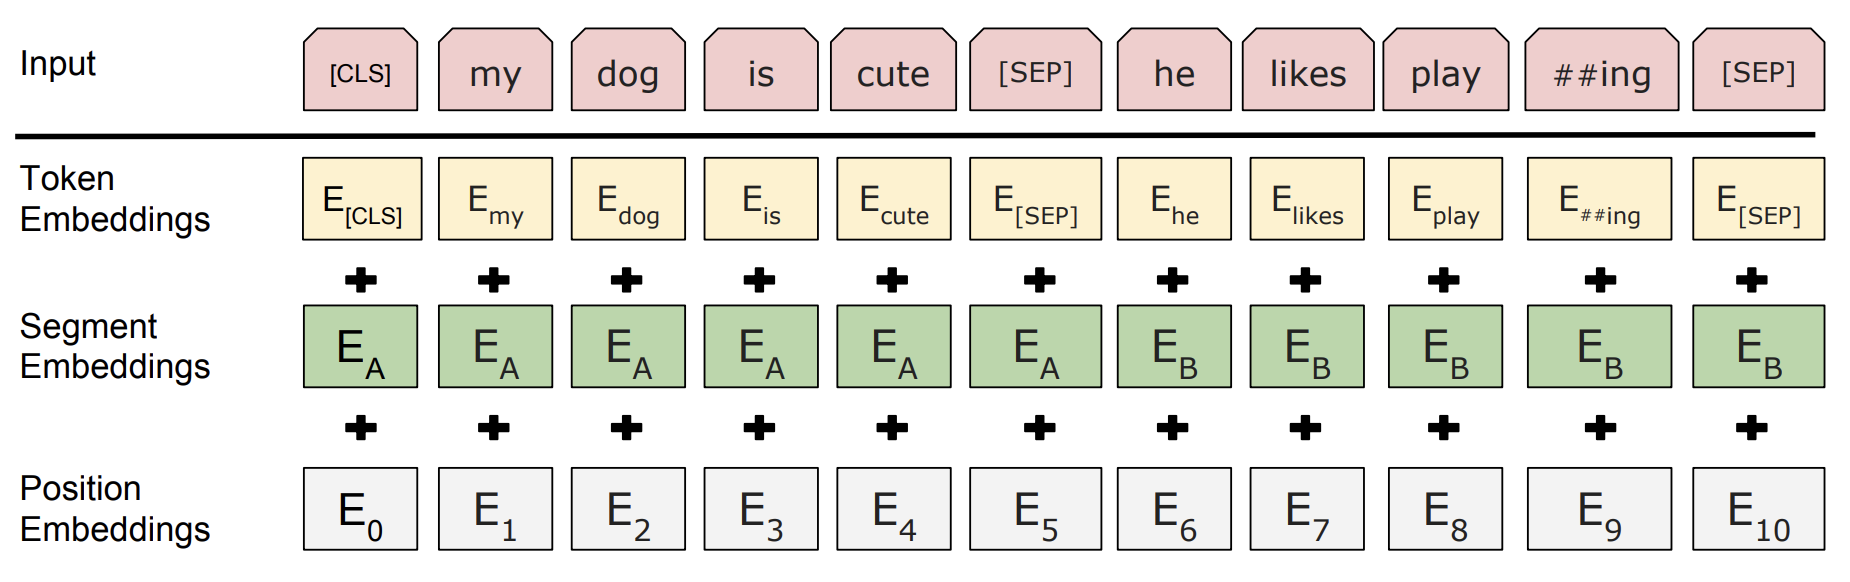
\includegraphics[width=\linewidth]{static/bert_tokenizierung.png}
        \caption{\label{fig:bert_tokenizierung} Zusammensetzung eines Input Tokens im BERT Modell \cite{devlin2019}}
    \end{center}
\end{figure}

Das Input Token ergibt sich aus dem Token-, Position- und Segment-Embedding. Das Position-Embedding (Position Encoding in Abbildung \ref{fig:transformeroverview}) 
stellt hierbei die jeweilige Position im Satz dar und das Segment-Embedding ordnet den Token dem entsprechenden Satz zu.

Vortrainiert wurde das BERT-Modell auf dem BookCorpus, einem Datensatz bestehend aus 11.038 unveröffentlichten Büchern, sowie auf der englischsprachigen Wikipedia 
(ohne Listen, Tabellen und Überschriften) \cite{DBLP:journals/corr/abs-1810-04805}.

\subsubsection{RoBERTa} \label{sec04:roberta}

Aufgrund der Annahme, dass das in Kapitel \ref{sec04:bert} beschriebene BERT Modell nicht ausreichend trainiert wurde, entwickelte 
\cite{DBLP:journals/corr/abs-1907-11692} das RoBERTa Modell.

Statt WordPiece nutzt RoBERTa Byte-Pair-Encoding (BPE) zum Tokenisieren wobei ein Vokabular von 50.265 Token verwendet wird.

BPE besteht aus folgenden, in \cite{sennrich2015} erklärten, Schritten:
\begin{enumerate}
  \item Zerlege jedes Wort in einzelne Zeichen und hänge ein Endsymbol „·“ an (z.\,B.\ \texttt{``lower''} → \texttt{[l, o, w, e, r, ·]}).
  \item Zähle alle benachbarten Zeichenpaare im Korpus (z.\,B.\ \texttt{(l,o)}, \texttt{(o,w)}, \texttt{(w,e)}, \dots).
  \item Führe das häufigste Paar zu einem neuen Symbol zusammen (z.\,B.\ \texttt{(l,o)} → \texttt{``lo''}).
  \item Wiederhole Schritt 2–3 für eine feste Anzahl von Merges (z.\,B.\ \texttt{``lo'' + ``w'' → ``low''} → \texttt{[low, e, r, ·]}).
  \item Speichere die entstandenen Merge-Regeln und wende sie auf neue Wörter an.
\end{enumerate}

Die Eingaben bestehen aus Abschnitten von 512 aufeinanderfolgenden Token, die sich auch über mehrere Dokumente erstrecken können. 
Der Beginn und das Ende eines Dokuments werden durch spezielle Markierungen <s> und </s> gekennzeichnet. 
Während des Pretrainings werden 15\% der Token maskiert – in 80\% der Fälle durch <mask>, in 10\% durch 
ein zufälliges anderes Token und in den restlichen 10\% bleiben sie unverändert. 
Anders als bei BERT erfolgt die Maskierung dynamisch, also in jeder Epoche neu.

Das RoBERTa-Modell wurde auf einer Zusammenführung von fünf Datensätzen vortrainiert: dem BookCorpus mit über 11.000 
unveröffentlichten Büchern, der englischen Wikipedia (ohne Listen, Tabellen und Überschriften), 
CC-News mit 63 Millionen englischsprachigen Nachrichtenartikeln aus dem Zeitraum September 2016 bis Februar 2019, 
OpenWebText als Open-Source-Rekonstruktion des WebText-Datensatzes von GPT-2 sowie dem Stories-Datensatz, 
einem nach erzählerischem Stil gefilterten Ausschnitt aus CommonCrawl-Daten. Insgesamt umfassen diese Datensätze 160 GB an Text.

\subsubsection{XML-RoBERTa} \label{sec04:xml_roberta}

Im Gegensatz zu RoBERTa, das ausschließlich auf englischen Texten trainiert wurde, ist XLM-RoBERTa ein mehrsprachiges 
Transformer-basiertes Sprachmodell, das auf 100 Sprachen trainiert wurde. 
Die Trainingsdaten umfassen über 2 Terabyte gefilterter CommonCrawl-Texte.
Auch die Vokabulargröße ist mit 250.002 Token deutlich größer als die 50.265 Token bei RoBERTa \cite{DBLP:journals/corr/abs-1911-02116}.

Statt Byte-Pair-Encoding (BPE) wie bei RoBERTa verwendet XLM-RoBERTa den SentencePiece Tokenizer.
Dieser arbeitet sprachunabhängig, benötigt keine vorab segmentierten Daten und funktioniert auch auf rohem Unicode-Text. 
Besonders wichtig ist das Konzept der lossless Tokenization, das Segmentierung vollständig reversibel macht \cite{kudo-richardson-2018-sentencepiece}.
Sentence Piece setzt sich aus vier Hauptkomponenten zusammen. Dem Normalizer, Trainer, Encoder und Decoder. 

\begin{enumerate}
    \item Der \textbf{Normalizer} wandelt unter anderem alle Zeichen in ASCII um, normalisiert Leerzeichen und ersetzt alle Groß- mit Kleinbuchstaben.
    \item Der \textbf{Trainer} erstellt aus diesen normalisierten Daten daraufhin ein Subwort-Modell. Jedes Subwort bekommt eine eindeutige ID.
    \textless s \textgreater markiert den Start eines Satzes und hat immer die ID 0. Das \_ steht für ein Leerzeichen und markiert somit den Wortanfang.
    \item Der \textbf{Encoder} kodiert nun einen übergebenen Input basierend auf dem erstellten Subwort-Modell in eine ID-Sequenz.
    item Der \textbf{Decoder} dekodiert eine erstellte ID-Sequenz zurück in einen lesbaren Input.
\end{enumerate}

In Kapitel \ref{sec04:bert} wurde bereits die Funktionsweise des MLMs erklärt. Die Erweiterung von MLM ist das Translation Language Model (TLM).
Im TLM werden statt einzelner Sätze (wie im MLM) übersetzte Satzpaare verwendet. Wörter in beiden Sprachen werden maskiert, und das Modell lernt, 
sie mithilfe beider Sprachversionen zu erraten (siehe Abbildung \ref{fig:translation_language_modeling}). So lernt es, die Bedeutungen über Sprachgrenzen hinweg zu 
verbinden.

\begin{figure}[htbp]
    \begin{center}
    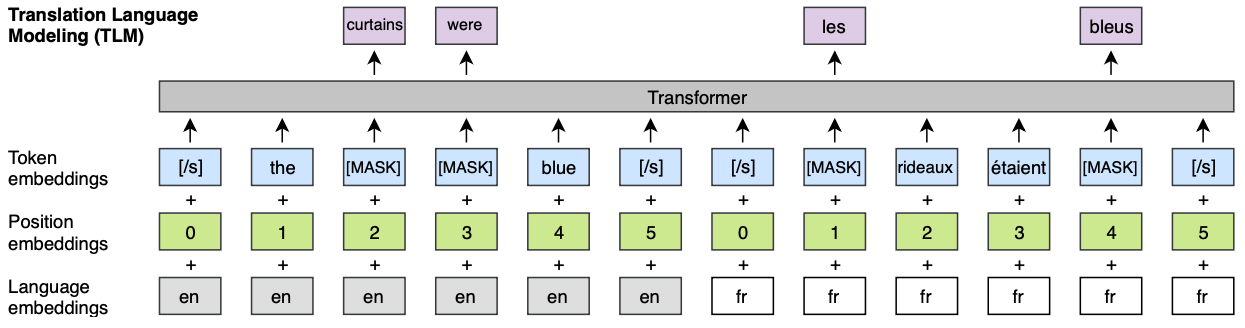
\includegraphics[width=\linewidth]{static/translation_language_modeling.png}
    \caption{\label{fig:translation_language_modeling} Auswertung eines bilingualen Satzpaares von TLM \cite{NEURIPS2019_c04c19c2}}
    \end{center}
\end{figure}

XLM ist ein mehrsprachiges Sprachmodell, das darauf ausgelegt ist, Sprachverständnis über mehrere Sprachen hinweg zu ermöglichen.
Vortrainiert wird es mit MLM und zusätzlich TLM.
Durch diese Kombination kann das Modell lernen, ähnliche Inhalte in verschiedenen Sprachen miteinander zu verknüpfen \cite{NEURIPS2019_c04c19c2}.